We consider a continuous spatial variable in $\mathbb{R}^1$ s.t. 
\begin{align*}
    \{r(x): x \in \text{D} &: [1,50] \subset \mathbb{R}^1\} \\
    \E\{r(x)\} &= \mu_r = 0\\
    \Var\{r(x)\} & = \sigma_r^2 \\
    \Corr\{r(x), r(x')\} & = \rho_r(\tau) \, ,
\end{align*}

where $\tau = |x-x^\prime|/10.$ 
Discretization: $\text{L} \in \{1,2,...,50\}$.
The discretized random field (RF) is 
\begin{equation*}
    \{r(x): x \in \text{L}\}.
\end{equation*}

\paragraph{a)}
A function $c(\vect{\tau}) : \R^q \rightarrow \R$ is positive definite (non-negative definite, to be precise) for $\vect{\tau} \in \R^q$ if
%
\begin{equation*}
\begin{split}
    & \sum_{i=1}^n \sum_{j=1}^n \alpha_i \alpha_j c(\vect{x_i} - \vect{x_j}) \geq 0 \\
    & \forall [\vect{x}_1, \vect{x}_2, \dots, \vect{x}_n] \in \R^{q \times n} \\
    & \forall \vect{\alpha} \in \R^n \\
    & \forall n \in \mathbb{N}_+ \setminus \{1\} \, .
\end{split}
\end{equation*}
%
In one dimension we replace the vectors $\vect{\tau}, \vect{x}_i$ and $\vect{x}_j$ with scalars $\tau, x_i$ and $x_j$.

Now assume that $\sum_{i=1}^n \sum_{j=1}^n \alpha_i \alpha_j \rho_r(\tau) < 0$ for some $[x_1, x_2, \dots, x_n]$, $\vect{\alpha}$ and $n$. Then
%
\begin{align*}
    \Var\left(\sum_{i=1}^n \alpha_i r(x_i)\right) 
    &= \sum_{i=1}^n \sum_{j=1}^n \alpha_i \alpha_j \Cov\{r(x_i), r(x_j)\} \\
    &= \sum_{i=1}^n \sum_{j=1}^n \alpha_i \alpha_j \sigma^2_r \Corr\{r(x_i), r(x_j)\} \\
    &= \sigma^2_r \sum_{i=1}^n \sum_{j=1}^n \alpha_i \alpha_j \rho_r(\tau) \\
    &< 0 \, .
\end{align*}
%
But the variance of a weighted sum of random variables is non-negative, so this is a contradiction. Thus the correlation function needs to be positive definite.

Two possible correlation functions, $\rho_r(\tau)$, the Powered exponential and the Matern. The functions take values for $\tau$, and a parameter $\nu_r$. Let $\nu_r \in \{1,3\}$ for the Matern function and $\nu_r \in \{1,1.9\}$ for Powered exponential. 

The correlation functions for each $\nu_r$ are shown in figure \ref{fig:corrfunc}. We see that the correlation is 1 for $\tau = 0$ and goes to 0 as $\tau$ increases for all the function and parameter configurations, as desired.

Cruical features for the spatial correlation function...?

\begin{figure}
    \centering
    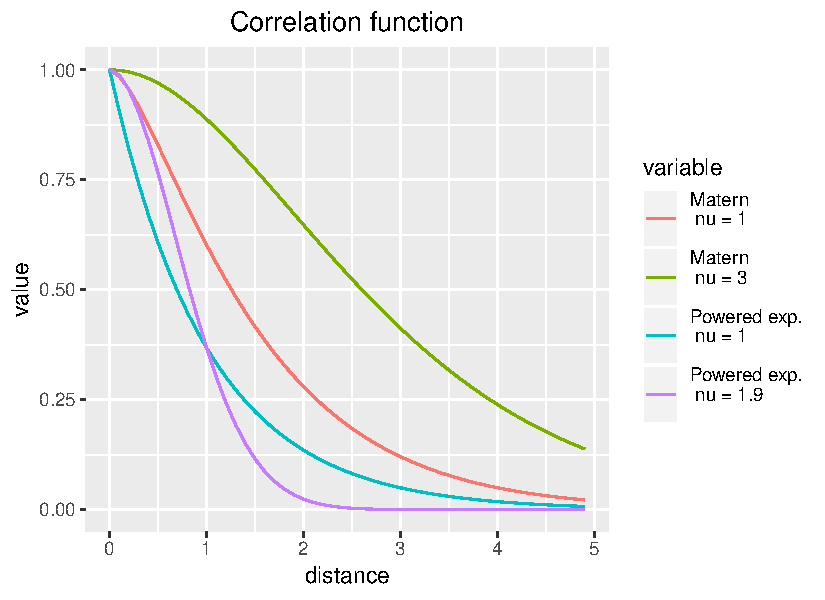
\includegraphics{figures/corrfunc.pdf}
    \caption{The Powered exponential and the Matern spatial correlation functions for some parameter values.}
    \label{fig:corrfunc}
\end{figure}

The variogram function is
%
\begin{align*}
\gamma_r(\tau)
\coloneqq&\: \frac{1}{2} \Var \{ r(x) - r(x') \} \\
=&\: \sigma_r^2 - \Cov\{r(x), r(x')\} \\
=&\: \sigma_r^2[1 - \rho_r(\tau)]\, ,
\end{align*}
%
i.e. 1 minus the correlation scaled by the variance.
This is displayed for the given parameter values in figure...

\begin{figure}
    \centering
    \includegraphics{figures/.pdf}
    \caption{The Powered exponential and the Matern spatial correlation functions for some parameter values.}
    \label{fig:corrfunc}
\end{figure}





%%%%%%%%%%%%%%%%%%%%%%%%%%%%%%%%%%%%%%%%%%%%%%%%%%%%%%%%%%%%%%%%%%%%%%
\paragraph{b)}
The discretized prior Gaussian model has pdf
\begin{equation}
    \vect{r} \sim p(\vect{r}) = \phi_n(\vect{r}; \mu_r \vect(i)_n, \sigma_r^2\matr{\Sigma}_r^{\rho}),
\end{equation}
where $n = 50$ is the number of grid points in $\text{L},$ $\vect{i}_n$ is a $n$-vector with $1$s and $\matr{\Sigma}_r^{\rho}$ is the correlation matrix for the grid points, defined from the chosen spatial correlation function applied to all $\tau$s in the system.

Ten realizations for each of the eight different parameter combinations are displayed in figures \ref{fig:prior_samp_exp} and \ref{fig:prior_samp_matern}. The priors in figure \ref{fig:prior_samp_exp} are using the Powered exponential function as correlation function, while the ones in figure \ref{fig:prior_samp_matern} use the Matern correlation function.

The influence of the parameter values are illustrated in the plots. Large $\sigma^2$ means large variability in values, and the realizations vary more along the $y$-axis in these displays. Increased $\nu_r$ increases the correlation between space points, as shown in figure \ref{fig:corrfunc}. Thus, this results in smoother realizations, where changes are done more gradually.

\begin{figure}[]
\centering
    \begin{subfigure}[H]{0.49\textwidth}
        \centering
        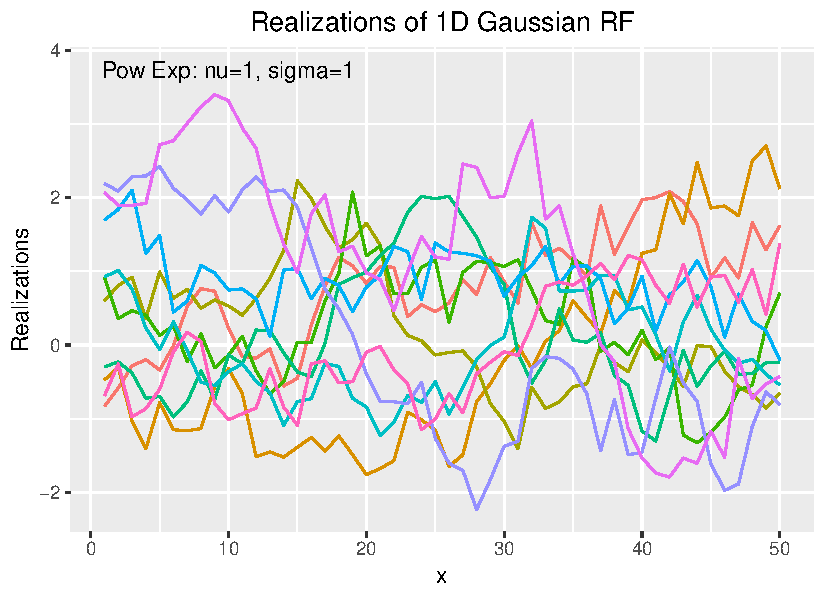
\includegraphics[scale=0.5,trim=0cm 0cm 0cm 0cm]{figures/sample1conf1.pdf}
    \end{subfigure}
    \hfill
    \begin{subfigure}[H]{0.49\textwidth}  
        \centering 
        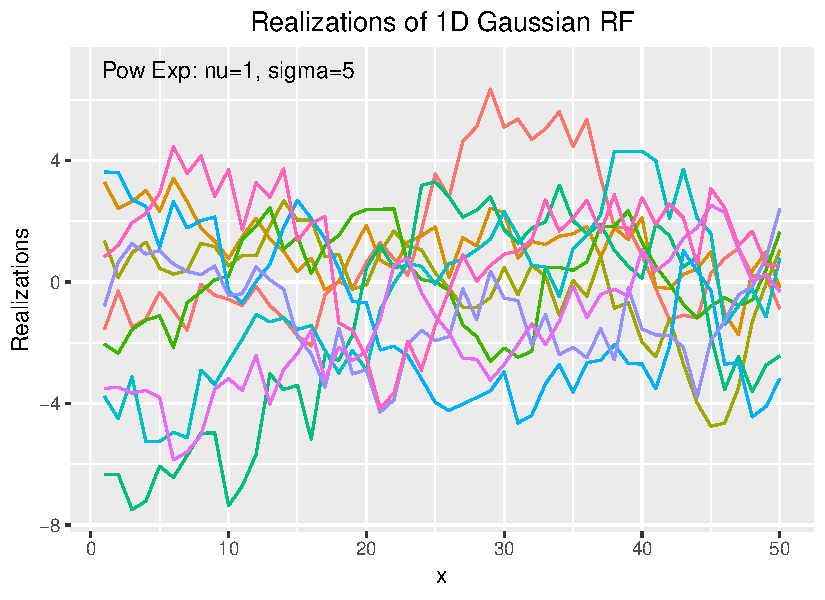
\includegraphics[scale=0.5,trim=0cm 0cm 0cm 0cm]{figures/sample1conf2.pdf}
    \end{subfigure}

    \vskip\baselineskip
    
     \begin{subfigure}[H]{0.49\textwidth}
        \centering
        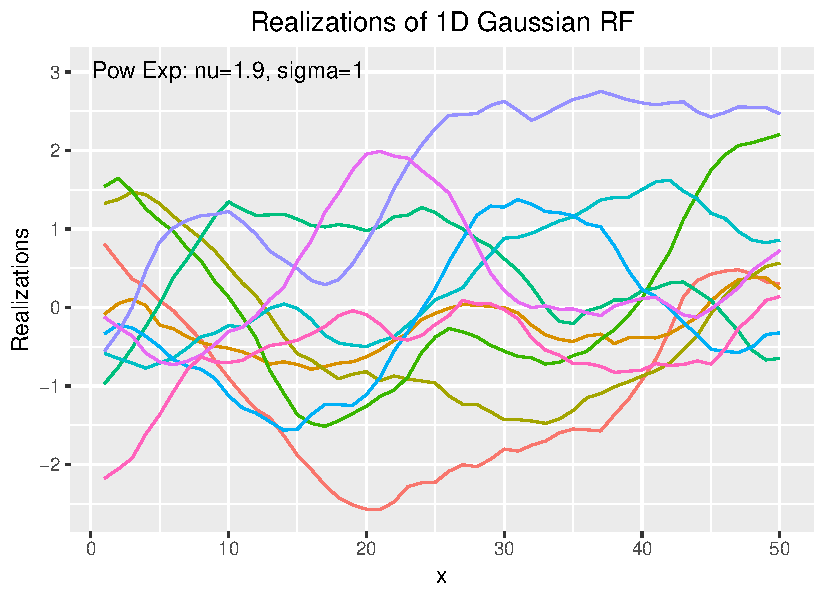
\includegraphics[scale=0.5,trim=0cm 0cm 0cm 0cm]{figures/sample1conf3.pdf}
    \end{subfigure}
    \hfill
    \begin{subfigure}[H]{0.49\textwidth}  
        \centering 
        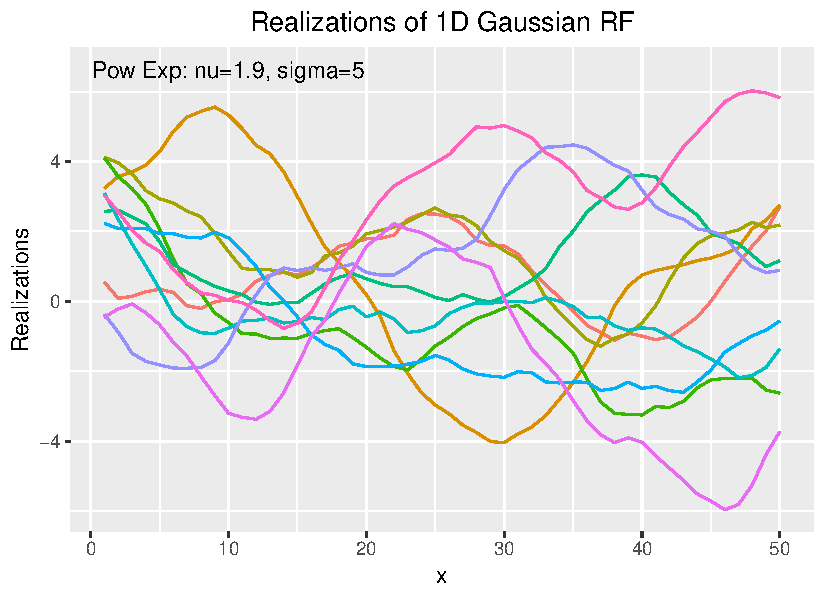
\includegraphics[scale=0.5,trim=0cm 0cm 0cm 0cm]{figures/sample1conf4.pdf}
    \end{subfigure}

    \caption{Realizations from prior Gaussian RF using Powered exponential correlation function. Model parametere values are shown the each plot, respectively.}
    \label{fig:prior_samp_exp}
\end{figure}

\begin{figure}[]
\centering
    \begin{subfigure}[H]{0.49\textwidth}
        \centering
        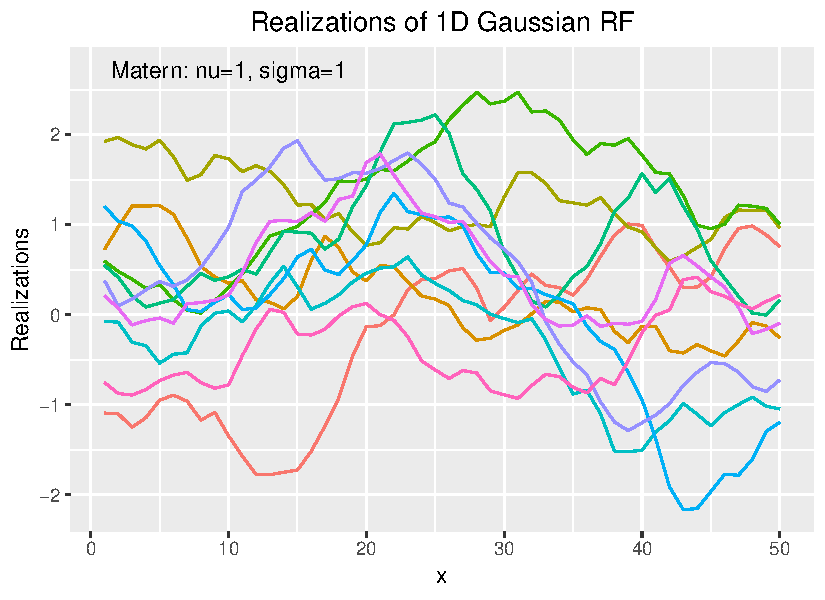
\includegraphics[scale=0.5,trim=0cm 0cm 0cm 0cm]{figures/sample1conf5.pdf}
    \end{subfigure}
    \hfill
    \begin{subfigure}[H]{0.49\textwidth}  
        \centering 
        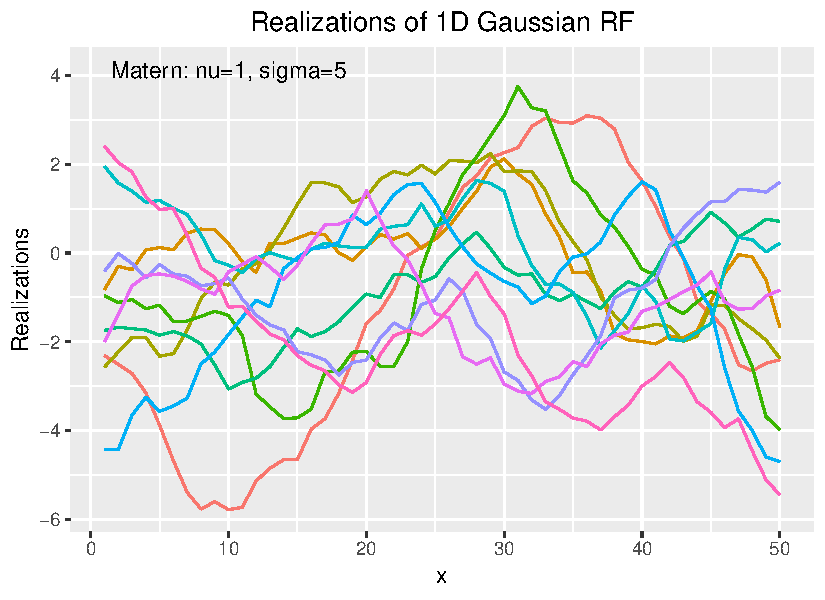
\includegraphics[scale=0.5,trim=0cm 0cm 0cm 0cm]{figures/sample1conf6.pdf}
    \end{subfigure}

    \vskip\baselineskip
    
     \begin{subfigure}[H]{0.49\textwidth}
        \centering
        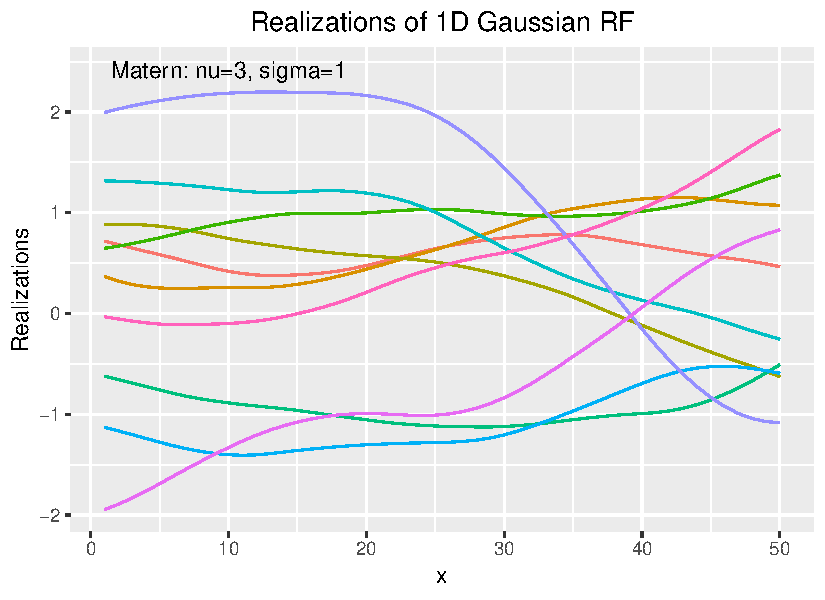
\includegraphics[scale=0.5,trim=0cm 0cm 0cm 0cm]{figures/sample1conf7.pdf}
    \end{subfigure}
    \hfill
    \begin{subfigure}[H]{0.49\textwidth}  
        \centering 
        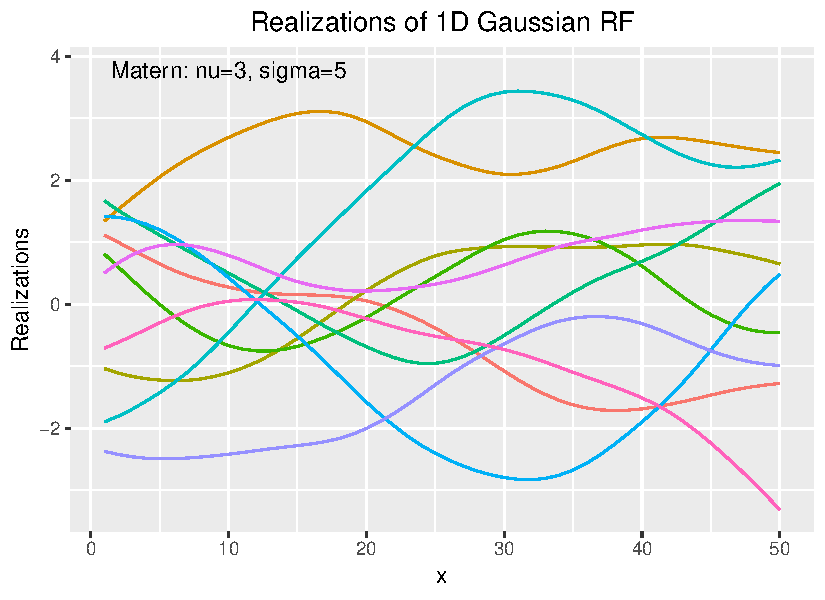
\includegraphics[scale=0.5,trim=0cm 0cm 0cm 0cm]{figures/sample1conf8.pdf}
    \end{subfigure}

    \caption{Realizations from prior Gaussian RF using Matern correlation function. Model parametere values are shown the each plot, respectively.}
    \label{fig:prior_samp_matern}
\end{figure}

%%%%%%%%%%%%%%%%%%%%%%%%%%%%%%%%%%%%%%%%%%%%%%%%%%%%%%%%%%%%%%%%%%%%%%
\paragraph{c)}
Now assume the spatial variable is observed as 
\begin{equation*}
    \{d(x): x \in \{10,25,30\} \subset \text{L} \}.
\end{equation*}
%%%%%%%%%%%%%%%%%%%%%%%%%%%%%%%%%%%%%%%%%%%%%%%%%%%%%%%%%%%%%%%%%%%%%%
\paragraph{d)}
text text text

%%%%%%%%%%%%%%%%%%%%%%%%%%%%%%%%%%%%%%%%%%%%%%%%%%%%%%%%%%%%%%%%%%%%%%
\paragraph{e)}
text text text

%%%%%%%%%%%%%%%%%%%%%%%%%%%%%%%%%%%%%%%%%%%%%%%%%%%%%%%%%%%%%%%%%%%%%%
\paragraph{f)}
text text text

%%%%%%%%%%%%%%%%%%%%%%%%%%%%%%%%%%%%%%%%%%%%%%%%%%%%%%%%%%%%%%%%%%%%%%
\paragraph{g)}
text text text
